\section{Methodology}
\label{sec:ch4-methodology}
This section outlines the research methodology used to investigate expert insights on biophilic design, detailing the interview design, participant selection, and data analysis approach.

\subsection{Expert Interviews}
We conducted semi-structured interviews, chosen for their flexibility to explore experts’ unique insights while maintaining a consistent structure across sessions~\cite{blandford2013semi}. A prepared ``interview guide'' outlined core areas of discussion with open-ended questions to encourage experts to be reflective and forward-thinking, while providing flexibility to tailor the conversations to their expertise. The conversations were organic, primarily driven by the experts' insights, with the guide serving as a loose framework to ensure relevance and depth, rather than dictating the flow of discussion. Ethical approval was obtained from the institutional review board. All experts provided verbal and written consent. Interviews were conducted in person or online, lasting 60–75 minutes.

\paragraph{Interview Design}
Conversations were loosely structured around experts’ context, grounded insights, experiential perspectives, and visionary outlooks---balancing practical inquiry with speculative thinking. \textbf{Context-setting} focused on situating experts within the framework of biophilic design while exploring their interpretations of its philosophy and its relevance within smart environments. \textbf{Grounded insights} explored practical design and engineering considerations, financial restrictions, technical challenges, and limitations. At this point, experts were invited to share their insights on  opportunities for incorporating the different sensory dimensions to foster immersive connections to nature. \textbf{Experiential perspectives} drew on personal stories and case studies where nature-inspired design created profound connections. Finally, \textbf{visionary outlooks} invited experts to imagine future biophilic spaces that respond to emerging human and ecological needs.

\begin{mainfigure}[tbp]
    \centering
    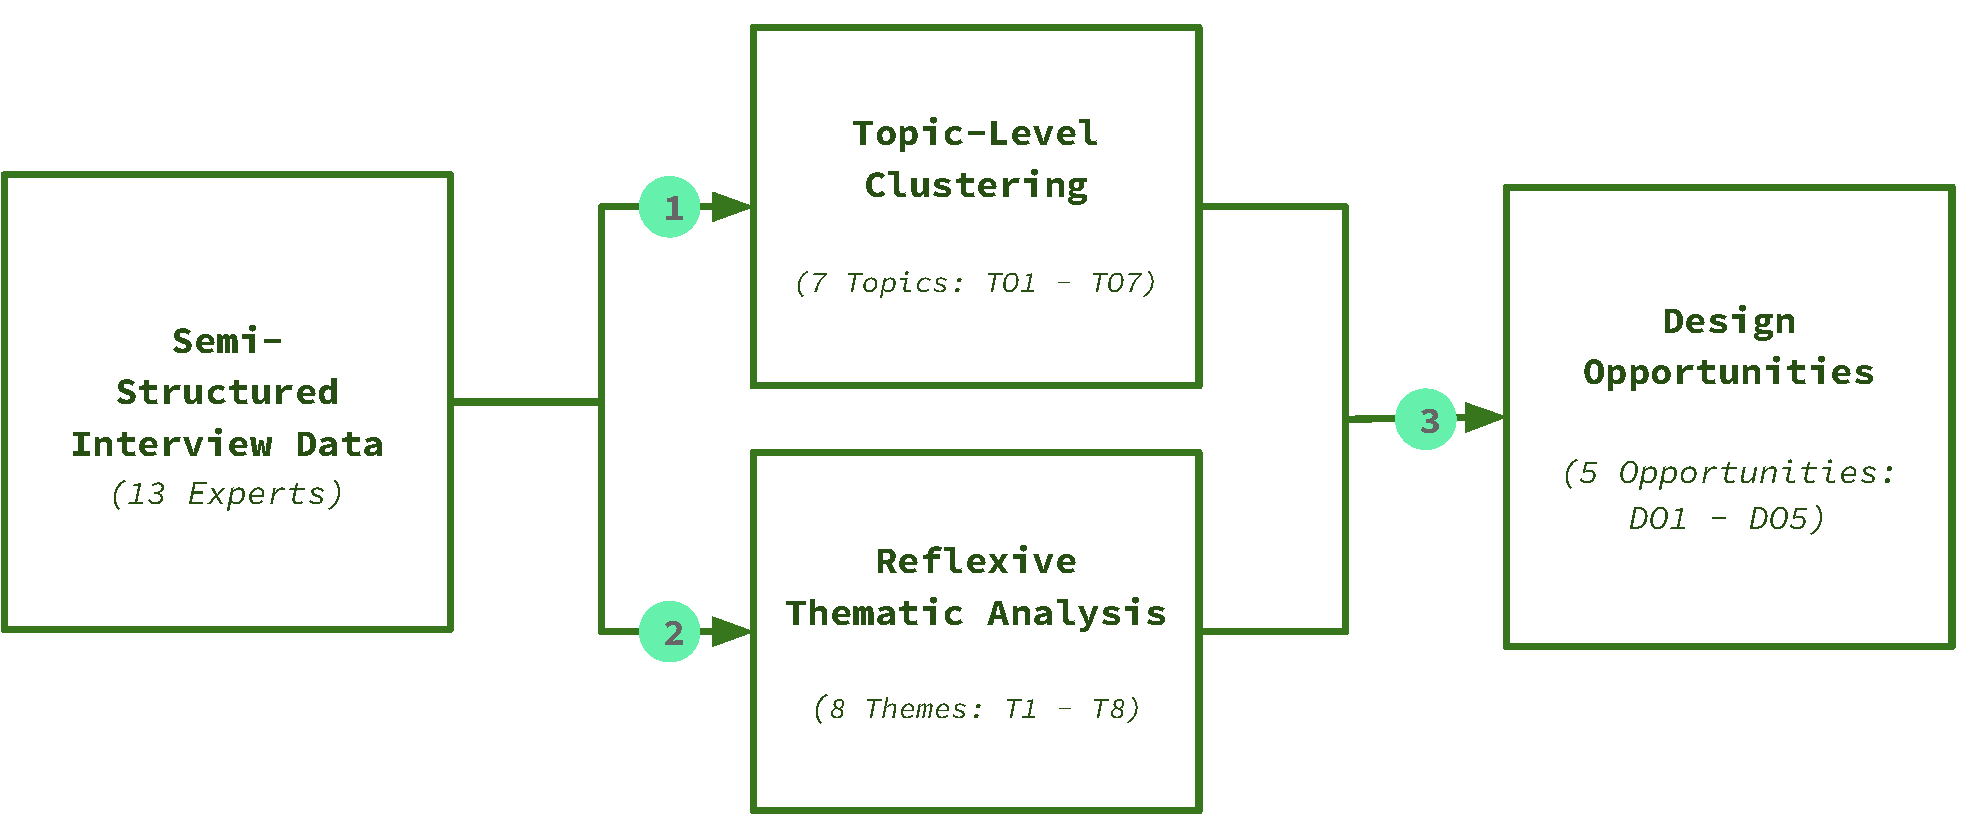
\includegraphics[width=0.9\linewidth]{images/ms-md-process-new.pdf}
    \caption{An overview of our data analysis process. First, we conducted topic-level clustering of interview responses, identifying seven descriptive topics based on recurring ideas across the interview questions. Next, we carried out a reflexive thematic analysis of the full dataset to generate eight themes. Finally, based on the topics and themes, we interpretively synthesised five design opportunities to support research on biophilic interaction in smart buildings.}
    \Description{A flowchart showing the three-stage analysis process of expert interviews. It begins with semi-structured interview data from 13 experts. Stage 1 is “Topic-Level Clustering,” resulting in 7 topics (TO1–TO7). Stage 2 is “Reflexive Thematic Analysis,” yielding 8 themes (T1–T8). Stage 3 is “Design Opportunities,” producing 5 opportunities (DO1–DO5). Arrows show a linear progression from data to topics, themes, and then opportunities.}
    \label{fig:md-md}
\end{mainfigure}

\subsection{Selection of Interviewees}
Experts were recruited via email through purposive sampling~\cite{serra2018social}. We reached out to individuals with significant contributions to biophilic design and related fields, including those affiliated with leading, global architecture firms, high profile architecture and design projects, as well as distinguished academic contributions. As the interviews progressed, snowball sampling was employed, leveraging existing experts’ networks to identify additional experts~\cite{raworth2012conducting}. In this way, we invited \textit{25} experts of which \textit{13} participated.  Among them, 8 were industry experts, including lead architects and senior designers (urban and landscape), while 5 were from academic backgrounds, comprising researchers specialising in interactive architecture and environmental psychology. A summary of participant demographics along with their stated expertise in biophilic design is provided in \autoref{appx-participant-demographics}.


\subsection{Data Processing and Analysis}
\label{sec:ch4-data-processing}
We conducted 13 expert interviews, resulting in approximately 17 hours of recorded audio, which were transcribed and analysed through a multi-stage process. Our analysis yielded findings at three levels: (1) topics summarising the interview data, (2) reflexively constructed themes around expert imaginaries in biophilic design, and (3) design opportunities. Figure~\ref{fig:md-md} summarises this process. 

\paragraph{Step 1 – Topic-Level Clustering of Expert Responses}
We began by organising the interview data using the structure of our interview questions (c.f. \autoref{appendix-outline} and discussed under Interview Design). We then grouped similar responses and identified recurring ideas. From these patterns, we developed a structured coding scheme (Figure~\ref{fig:findings-findings-overview}) comprising high-level topics such as \textit{values}, \textit{deeper connection}, and \textit{technology}. These topics summarise expert discourse and surface the breadth of insights across the interviews, reflecting a high-level, descriptive structuring of the dataset.


\paragraph{Step 2 - Reflexive Thematic Analysis}
Next, to elicit deeper insights from the dataset, we conducted a bottom-up reflexive thematic analysis following \citet{braun2023thematic, byrne2021worked}, which allowed for an iterative and open coding process. Reflexive thematic analysis was chosen for its effectiveness in identifying and interpreting patterns across datasets, particularly in under-researched areas~\cite{clarke2013successful, braun2013shouldn}. This analysis was conducted independently of Step 1, where we returned to the full dataset and carried out line-by-line coding of the transcripts. Each sentence was examined with attention to both semantic and latent meaning, yielding $471$ open codes (e.g. \textit{``spirit of the place'', ``participatory stewardship of nature'', ``biophilic design as corporate culture''}). These codes were iteratively reviewed and refined to create themes that reflect the possibilities of biophilic design, as articulated by the experts. 

\paragraph{Step 3 – Deriving Design Opportunities}
Finally, we engaged in an interpretive synthesis to develop design opportunities for interaction design in smart environments. This process drew from the structured topics (Step 1) and reflexive themes (Step 2), re-examining the findings through our designerly and technological lens. For each opportunity, we also proposed speculative technology examples using “what if?” scenarios to explore how biophilic interaction might be reimagined.

Throughout the study, the first and last author discussed and resolved methodological and analytical decisions. The first author identified high-level topics based on the transcripts, which were then reviewed and refined (Step 1). The first author then conducted open coding and theme development, with codes and developed themes discussed and adjusted in joint meetings (Step 2). Finally, the first and the last author iteratively reviewed and shaped the design opportunities (Step 3). 





